\chapter{Background}\label{chap:background}
\section{The Mass Balancing Problem}

\begin{figure}
    \centering
    \usetikzlibrary{arrows.meta,3d}
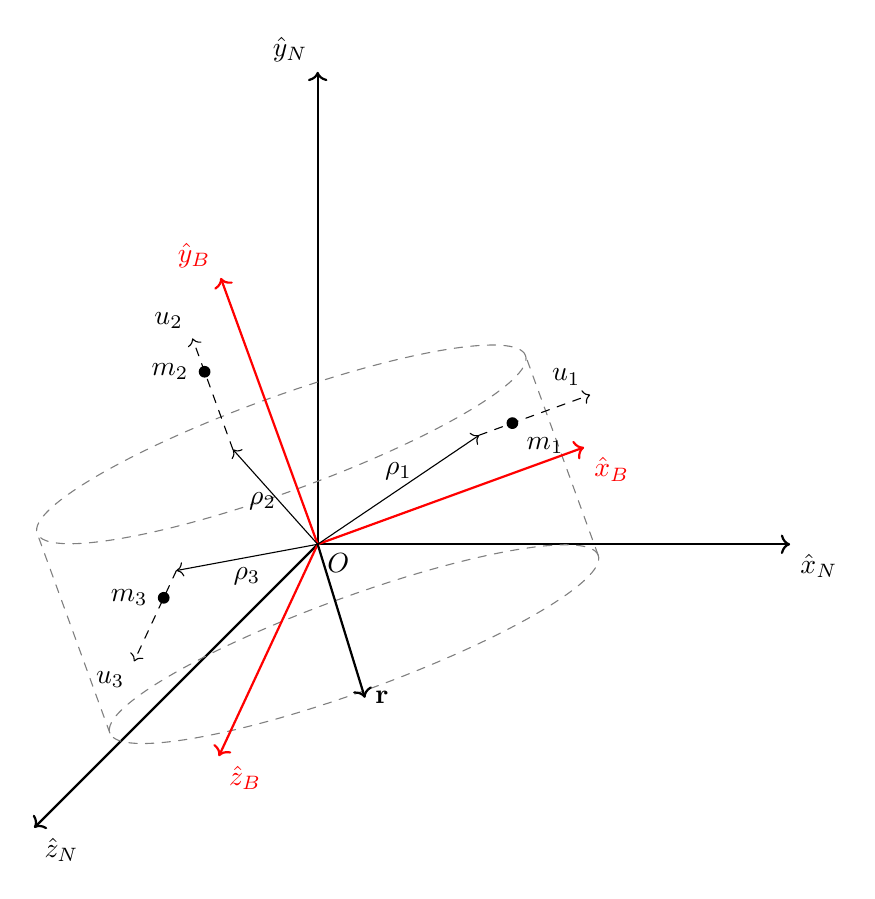
\begin{tikzpicture}[scale=3, line cap=round, line join=round]

% Inertial frame (I)
\draw[->, thick] (0,0) -- (2,0) node[below right] {$\hat{x}_N$};
\draw[->, thick] (0,0) -- (0,2) node[above left] {$\hat{y}_N$};
\draw[->, thick] (0,0) -- (-1.2,-1.2) node[below right] {$\hat{z}_N$};
\node[below right] at (0,0) {$O$};

% Cylinder representing platform ------------------------------
\pgfmathsetmacro{\radius}{1.1}
\pgfmathsetmacro{\height}{0.9}

\begin{scope}[rotate around={20:(0,0)}] 
    \draw[gray,dashed] (0,-\height/2) ellipse ({\radius} and 0.2);
    \draw[gray,dashed] (0,\height/2) ellipse ({\radius} and 0.2);
    \draw[gray,dashed] (-\radius,-\height/2) -- (-\radius,\height/2);
    \draw[gray,dashed] (\radius,-\height/2) -- (\radius,\height/2);
\end{scope} 

% Body frame (B), shifted and rotated
\begin{scope}[rotate=20]
    \draw[->, thick, red] (0,0) -- (1.2,0) node[below right] {$\hat{x}_B$};
    \draw[->, thick, red] (0,0) -- (0,1.2) node[above left] {$\hat{y}_B$};
    \draw[->, thick, red] (0,0) -- (-0.7,-0.7) node[below right] {$\hat{z}_B$};
    % \node[below left, red] at (0,0) {$\mathcal{B}$};

    % START M2 --------------------------------------
    \draw[->] (0,0) -- (-0.2,0.5) coordinate (rho2_end) 
        node[pos=0.65, below] {$\rho_2$};

    \draw[->, dashed] (rho2_end) -- ++(0,0.5) coordinate (u2_end)  
        node[above left] {$u_2$};

    \path (rho2_end) -- (u2_end) 
        node[pos=0.7, circle, fill=black, inner sep=1.5pt, label=left:$m_2$] {};

    % START M1 --------------------------------------
     \draw[->] (0,0) -- (0.8,0.2) coordinate (rho1_end) 
        node[midway, above] {$\rho_1$};

    \draw[->, dashed] (rho1_end) -- ++(0.5,0) coordinate (u1_end)  
        node[above left] {$u_1$};

    \path (rho1_end) -- (u1_end) 
        node[pos=0.3, circle, fill=black, inner sep=1.5pt, label=below right:$m_1$] {};

    % START M3 -----------------------------------
    \draw[->] (0,0) -- (-0.6,0.1) coordinate (rho3_end) 
        node[midway, below] {$\rho_3$};

    \draw[->, dashed] (rho3_end) -- ++(-0.3,-0.3) coordinate (u3_end)  
        node[below left] {$u_3$};

    \path (rho3_end) -- (u3_end) 
        node[pos=0.3, circle, fill=black, inner sep=1.5pt, label=left:$m_3$] {};
\end{scope}

% START COM r ----------------------------------
\draw[->, thick] (0,0) -- (0.2, -0.65) coordinate (r_end)
    node[below, right] {$\mathbf{r}$};
 




\end{tikzpicture}
    \caption{The mass balancing problem for air bearing based spacecraft dynamics simulators}
    \label{fig:mbs_problem}
\end{figure}


\Cref{fig:mbs_problem} defines the geometery of the problem in a general case. $O$ represents the common origin of the inertial frame $\mathcal{N}$ and the body-fixed principle frame of the simulator $\mathcal{B}$. $O$ is chosen to be the center of rotation . If frictionless rotation is assumed, then the simulator follows Euler's rotational equations of motion with gravity acting as a torque. 

\begin{equation}
    \bm{J}\,\dot{\bm{\omega}} + \bm{\omega}^{\times}\,\bm{J}\bm{\omega} = \bm{T}_g
\end{equation}

Here, $\bm{J}$ is the inertia of the simulator about $O$, $\bm{\omega}$ is the angular velocity of the simulator, and $\bm{T}_g$ is the torque due to gravity. $\dot{\bm{v}}$ represents the time derivative of some vector $\bm{v}$, and $\bm{v}^{\times}$ represents the skew-symmetric cross-product matrix of $\bm{v}$. All vectors and inertias are expressed in $\mathcal{B}$. In general it is more convienent to expand $\bm{T}_g$ which leads to

\begin{equation}\label{equation:starting_eom}
    \bm{J}\,\dot{\bm{\omega}} + \bm{\omega}^{\times}\,\bm{J}\bm{\omega} = m_s\bm{r}^{\times}\bm{g}
\end{equation}

where $m_s$ is the total mass of the simulator, $\bm{r}$ is the center of mass relative to $O$, and the $\bm{g}$ is the accleration due to gravity.

\textit{NEED A NOTE ABOUT Jdot and R i dot being approximated to zero}
\Cref{fig:mbs_problem} also shows the introduction of three sliding masses, although in general there may be as many as $n$ sliding masses. Each mass $m_i$ has one translational degree of freedom along $\bm{u}_i$, and $\bm{\rho}_i$ represents the position of the $i$-th mass in it's homed position. Since in practice each mass can only travel some limited distance along $\bm{u}_i$, the homed position of a mass is defined as the center of this range of positions. The position relative to $O$ of any mass $\bm{R}_i$ can be obtained with 
\begin{equation}\label{equation:sliding masses}
    \bm{R}_i = \bm{\rho}_i + d_i\bm{u_i}
\end{equation}
where $d_i$ is the distance a mass $m_i$ has travelled along $u_i$ relative to it's zeroed position. More generally, $\Delta\,d_i$ is defined as the change in position a mass from any arbitrary starting position.

Additionally, $\bm{R}_i$ may change with time, say through linear actuators. It will be assumed the linear actuators have some form of absolute positioning, or that they can command the masses to their homed positions in a repeatable way. Let $\bm{J}_0$ be the total inertia of the simulator with the masses in their homed positions. The inertia as a function of time is then 
\begin{equation}
    \bm{J}(t)=\bm{J}_0-\sum_{i=0}^{n}(m_i\bm{R}_i^{\times}(t)\bm{R}_i^{\times}(t)-\bm{\rho}_i^{\times}\bm  {\rho}_i^{\times})
\end{equation}
The sliding mass will also introduce angular momentum into the system, which can be calculated using 
\begin{equation}
    \bm{h}_m =\sum_{n}^{i=1}\bm{R}_i^{\times}m_i\dot{\bm{R}}_i^{\times}
\end{equation}
In practical mass balancing applications however, the mass of each block is very small relative to the overall mass of the simulator. If a reasonable attempt is made to balance the simulator manually beforehand, then the masses will also move slowly and over short distances. This allows the following simplications to be made
\begin{equation}
\bm{J}(t) \approx \bm{J}_0 \Longrightarrow \dot{\bm{J}}=\bm{0}
\end{equation}
\begin{equation}\label{equation:h_m_eq_0}
\dot{\bm{R}}_i \approx \bm{0} \Longrightarrow \bm{h}_m=\bm{0}
\end{equation}

The goal of these definitions is to obtain an equation relating how changing the positions of each mass effects the center of mass of the total system. These parameters are first assembled into matricies as follows

\begin{equation}
    \bm{M}=\mathrm{diag}(\frac{m_1}{m_s}, \cdots  ,\frac{m_n}{m_s}) \in \mathbb{R}^{n \times n}
\end{equation}
\begin{equation}
    \bm{U}=
    \begin{bmatrix}
        \bm{u}_1, & \cdots & ,\bm{u}_n
    \end{bmatrix}
    \in \mathbb{R}^{3 \times n}
\end{equation}
\begin{equation}
    \Delta\bm{d}=
    \begin{bmatrix}
        \Delta\,d_1, & \cdots & ,\Delta\,d_n 
    \end{bmatrix}^T
    \in \mathbb{R}^{n}
\end{equation}

Using these defintions, writing $\Delta\bm{r}$ as a function of $\Delta\bm{d}$ becomes a simple matrix multiplication

\begin{equation}
    \Delta\bm{r} = \bm{U}\bm{M}\Delta\bm{d}
\end{equation}
 
This means the value of $\bm{r}$ at any point can be written as $\bm{r}=\bm{r}_0+\Delta\bm{r}$, where $\bm{r}_0$ is the center of mass with the masses in their homed positions. An equally important relation is writing $\Delta\bm{d}$ as a function of $\Delta\bm{r}$. For the case $n = 3$ with linearly independent values of $\bm{u}_i$, the unique solution is given by
\begin{equation}\label{equation:delta_d_sol}
    \Delta\bm{d} = (\bm{U}\bm{M})^{-1}\Delta\bm{r}
\end{equation}
If $n>3$, a solution that minimizes the mass moved can be found using a pseudoinverse approach
\begin{equation}\label{equation:delta_d_pseudo_sol}
    \Delta\bm{d} = (\bm{U}\bm{M})^{\dagger }\Delta\bm{r}
\end{equation}

where $(\bm{U}\bm{M})^{\dagger}$ represents the Moore-Penrose pseudoinverse of $\bm{UM}$.

There are two main approaches to solving the mass balancing problem. The first is to hold the mass positions constant and obtain an estimate of the value of $\bm{r}$, denoted as $\hat{\bm{r}}$. The required change in positions of the sliding masses are then applied all at once. The exact values are calculated from \Cref{equation:delta_d_sol} or \Cref{equation:delta_d_pseudo_sol}, substituting $-\hat{\bm{r}}$ for $\Delta\bm{r}$. This class of approaches is referred to passive balancing, offline balancing, or the batch estimation method.

The second main approach is to find a feedback control law that drives the effect of the $m_s\bm{r}^{\times}\bm{g}$ term in \Cref{equation:starting_eom} to zero. In traditional spacecraft ADCS, the torques required for a feedback controller are generated using momenutum exchange devices, but here, there is the additional option to use $\Delta\bm{d}$ as a control input. Referring to \Cref{equation:starting_eom}, the dynamics of the system are influenced by the value of $\bm{r}^{\times}$, whose value can be controlled by $\Delta\bm{d}$ using \Cref{equation:delta_d_sol} or \Cref{equation:delta_d_pseudo_sol}. This class of approaches is referred to as active balancing or feedback control balancing.

Once any balancing procedure has been performed, it is important to verify the results through an external verification method. Assuming the center of mass is below the center of rotation, a very rough estimate for the torque due to gravity may be obtained by tilting the simulator about one of it's principal axes, releasing it, and observing the period of resulting pendulum motion $T$ \cite{kim_automatic_2009}. The relationship between $\bm{r}$ and $T$ is given by
\begin{equation}
    T = 2\pi\sqrt{\frac{J_i}{m_s\,g||\bm{r}||}}
\end{equation}
where $J_i$ is the moment of inertia about said principle axis. After performing a balancing procedure, the value of $||\bm{r}||$ should decrease, leading to longer periods of oscillatation. 

Another verification method is observing the total mechanical energy of the simulator while it undergoes this same pendulum motion. The mechanical energy is given by
\begin{equation}
    E_{mech} = \frac{1}{2}\bm{\omega}^T\bm{J}\bm{\omega} + mgh
\end{equation}
where $h$ is the vertical height of $\bm{r}$ \cite{silva_filtering_2018}. If the simulator is balanced, $h$ will remain relatively constant throughout the pendulum motion, and the kinetic energy term $\frac{1}{2}\bm{\omega}^T\bm{J}\bm{\omega}$ will also remain relatively constant due to the conservation of energy. As the balance of the simulator improves, the kinetic energy will oscillate with smaller amplitudes.

Ideally this value is zero, but in practice mass balancing systems seek to make this value as small as possible while satsifying other project constraints like cost, time, and volume. 

\section{Mass Balancing Hardware}

\section{Batch Estimation Algorithms}

Batch estimation algorithms are a subset of passive balancing methods that use momentum exchange devices to excite the simulator and record the resulting body rate and attitude data. The equations of motion are manipulated to help obtain multiple estimates of $\bm{r}$, and a single, final estimate of $\bm{r}$ is calculated using least-squares error methods. Many variations of batch estimation algorithms exist, but they all start with same principle up seperating the constant mass properties from the dynamic states in the equations of motion. To accomplish this, it helps to define the following variables

\begin{equation}
    \bm{\Omega} =
        \begin{bmatrix}
            \omega_1 & 0 & 0 & -\omega_2 & -\omega_3 & 0 \\
            0 & \omega_2 & 0 & -\omega_1 & 0 & -\omega_3 \\
            0 & 0 & \omega_3 & 0 & -\omega_1 & -\omega_2
        \end{bmatrix}
\end{equation}
\begin{equation}
    \bm{x} = \begin{bmatrix}
        J_{xx} & J_{yy} & J_{zz} & J_{xy} & J_{xz} & J_{yz} & m_s\,r_x & m_s\,r_y & m_s\,gr_z
    \end{bmatrix}^T
\end{equation}

Using these values, the original equations of motion in \Cref{equation:starting_eom} can be rewritten as 
\begin{equation}\label{equation:no_MEDs}
    \begin{bmatrix}
        \dot{\bm{\Omega}}+\bm{\omega}^{\times}\bm{\Omega} & \bm{g}^{\times}
    \end{bmatrix}\bm{x}
    =\bm{0}
\end{equation}
with the goal being to eventually solve for $\bm{x}$. To avoid nullspace solutions (which give physically invalid mass properties), additional terms must be introduced to the right hand side. This is done through the use of momentum exchange devices which changes \Cref{equation:no_MEDs} into 
\begin{equation}\label{equation:with_MEDs}
    \begin{bmatrix}
    \dot{\bm{\Omega}}+\bm{\omega}^{\times}\bm{\Omega} & \bm{g}^{\times}
    \end{bmatrix}\bm{x}
    =-\dot{\bm{h_c}} - \bm{\omega}^{\times}\bm{h_c}
\end{equation}

where $\bm{h}_c$ represents the total angular momentum of the MEDs. Additionally, to avoid taking the numerical derivative of the noisy signal $\bm{\omega}$ (which will come from gyroscopes), both sides of \Cref{equation:with_MEDs} are integrated with resepct to time which results in 
\begin{equation}\label{equation:LSM_no_k}
    \begin{bmatrix}
    \int_{t_0}^{t}\dot{\bm{\Omega}}+\bm{\omega}^{\times}\bm{\Omega}\,dt & \int_{t_0}^{t}\bm{g}^{\times}\,dt
    \end{bmatrix}\bm{x}
    =-{\bm{h_c}} - \int_{t_0}^{t}\bm{\omega}^{\times}\bm{h_c}\,dt
\end{equation}

For each timestep $k$ where a measurement is taken, a new $\bm{A}$ and $\bm{T}$ matrix are created using
\begin{equation}
    \bm{A}_k=\begin{bmatrix}
    \int_{t_0}^{t_k}\dot{\bm{\Omega}}+\bm{\omega}^{\times}\bm{\Omega}\,dt & \int_{t_0}^{t_k}\bm{g}^{\times}\,dt
    \end{bmatrix}
\end{equation}
\begin{equation}
    \bm{T}_k=-{\bm{h_c}} - \int_{t_0}^{t}\bm{\omega}^{\times}\bm{h_c}\,dt
\end{equation}
which allows \Cref{equation:LSM_no_k} to be rewritten as 
\begin{equation}\label{equation:LSM_with_k}
    \bm{A}_k\bm{x}=\bm{T}_k
\end{equation}

Since all measurements are corrupted by noise, there will not be any single value of $\bm{x}$ that will satisfy \Cref{equation:LSM_with_k} for all $k$. Instead, the key idea with least squares estimation methods is to find a value of $\bm{x}$ that minimizes the error in \Cref{equation:LSM_with_k} across all $k$. The most common way to achieve is this to create augmented versions of $\bm{A}$ and $\bm{T}$ as
\begin{equation}
    \bar{\bm{A}}=\begin{bmatrix}
        \bm{A}_0 & \bm{A}_1 & \cdots & \bm{A}_n
    \end{bmatrix}\in \mathbb{R}^{3n \times 9}
\end{equation}
\begin{equation}
    \bar{\bm{T}}=\begin{bmatrix}
        \bm{T}_0 & \bm{A}_1 & \cdots & \bm{T}_n
    \end{bmatrix}\in \mathbb{R}^{3n \times 1}
\end{equation}
where $n$ is the total number of measurements. $\bm{x}$ is finally computed using 
\begin{equation}
    \bm{x}=\bar{\bm{A}}^{\dagger}\bar{\bm{T}}
\end{equation}
The offline batch estimation method requires that multiple tests are run, adjusting the sliding masses after each run using \Cref{equation:delta_d_sol} or \Cref{equation:delta_d_pseudo_sol}. Assuming actuators like reaction wheels are available, this method's main advantage is it's ease of implementation. By doing all of the estimation and data processing offline, no custom software needs to be written for the simulator's onboard computer. In fact, exciting the system using this method does not require the simulator to have a working feedback controller, allowing this method to be adopted early in the design of a simulator. Researches have demonstrated success using simple open loop control to ensure that the body rates of the simulator follow a sinusoidal pattern \cite{kim_automatic_2009} \cite{dam_applied_2014} \cite{noauthor_designing_2003}.



\section{Kalman Filtering for Inbalance Estimation}

Kalman filters have extensive precedent for estimating unknown parameters in dynamic systems for aerospace applications. In traditional spacecraft attitude determination and control, the Extended Kalman Filter is the primary method for determining spacecraft body rates and attitude. While a general derivation of the Kalman filter and its' variations is beyond the scope of this thesis, a brief background of it's application in spacecraft ADCS is important. Here, the state vector of the system is formulated as
\begin{equation}\label{equation:EKF_state_vec}
    \bm{x} = \begin{bmatrix}\bm{\omega} \\ \bm{q} \end{bmatrix}
    =\begin{bmatrix}
        \bm{\omega} \\ \eta \\ \bm{\epsilon}
    \end{bmatrix}
\end{equation}
where $\bm{q}$ represents the spacecraft's attitude in the form of a quaternion. In this work, $\bm{q}$ is defined as a frame rotation from the body frame to the inertial frame, with the real part $\eta$ of the quaternion first. The spacecraft quaternion at any point may be directly converted into a direction cosine matrix using the following
\begin{equation}
    \bm{C}_{\mathcal{N}\leftarrow\mathcal{B}}(\bm{q})=
    \begin{bmatrix}
    2q_0^{2}+2q_1^{2}-1 & 2(q_1 q_2 + q_0 q_3) & 2(q_1 q_3 - q_0 q_2) \\
    2(q_1 q_2 - q_0 q_3) & 2q_0^{2}+2q_2^{2}-1 & 2(q_2 q_3 + q_0 q_1) \\
    2(q_1 q_3 + q_0 q_2) & 2(q_2 q_3 - q_0 q_1) & 2q_0^{2}+2q_3^{2}-1
    \end{bmatrix}
\end{equation}
where $\bm{C}_{\mathcal{N}\leftarrow\mathcal{B}}$ again represents the frame rotation from $\mathcal{B}$ to $\mathcal{N}$. This means $\bm{C}_{\mathcal{N}\leftarrow\mathcal{B}}$ satisfies the following properties
\begin{equation}
    \bm{v}^{\mathcal{N}} = 
    \bm{C}_{\mathcal{N}\leftarrow\mathcal{B}}\bm{v}^{\mathcal{B}}
\end{equation}
\begin{equation}
    \bm{v}^{\mathcal{B}} = 
    \bm{C}_{\mathcal{N}\leftarrow\mathcal{B}}^T\bm{v}^{\mathcal{N}}
    =\bm{C}_{\mathcal{B}\leftarrow\mathcal{N}}\bm{v}^{\mathcal{N}}
\end{equation}
where $\bm{v}^{\mathcal{B}}$ represents some physical vector expressed in $\mathcal{B}$ and $\bm{v}^{\mathcal{N}}$ represents the same vector expressed in $\mathcal{N}$. In the standard EKF for spacecraft ADCS, the system state must be discretely propagated forward at each iteration. This is always done through some form of numerical integration, such as
\begin{equation}\label{equation:forward_euler}
    \bm{x}_{k} = \bm{x}_{k-1}+T\bm{f}(\bm{x}_{k-1},\bm{u}_{k-1})
\end{equation}
where $T$ is the discrete sample period, $k$ is the iteration number, and $\bm{u}$ is the control input. \Cref{equation:forward_euler} uses forward Euler integration, but higher-order schemes may also be used. Using quaternion kinematics, an exact expression for $\bm{f}$ can be derived which results in
\begin{equation}
    \bm{f}(\bm{x}_{k-1})=
    \begin{bmatrix}
    
    \bm{J}^{-1}(-\bm{\omega}_{k-1}^{\times}\bm{J}\bm{\omega}_{k-1})+\bm{u}_{k-1} \\

    -\frac{1}{2}\bm{\epsilon}_{k-1}^T\bm{\omega}_{k-1} \\

    \frac{1}{2}(\eta_{k-1}\mathbb{1} +
    \bm{\epsilon}_{k-1}^{\times})\bm{\omega}_{k-1}

    \end{bmatrix}
\end{equation}
where $\bm{\omega}_{k-1}$, $\bm{\epsilon}_{k-1}$, and $\eta_{k-1}$ are all taken directly from $\bm{x}_{k-1}$ according to \Cref{equation:EKF_state_vec}. Next, the propagated state is corrected using a set of measurements $\bm{y}$. These traditionally come from a variety of sensors, namely star trackers, magnetometers, and sun sensors. All of these work as valid measurements provided there is some function that can transform the system state into a measurement using $\bm{y} = \bm{h}(\bm{x})$. The process function and measurement function $\bm{f}$ and $\bm{h}$ may then be used to implement a variety of variations of the Kalman filter to obtain estimates of the state in the presence of process noise and measurement noise.



Multiple researchers have extended this to estimate the inbalance vector $\bm{r}$. To do this, the state vector of the dynamic system is written as 
\begin{equation}
    \bm{x} = \begin{bmatrix} \omega_x & \omega_y & \omega_z & r_x & r_y & r_z \end{bmatrix}^T
\end{equation}
and the associated dynamics of the system becomes
\begin{equation}
    \dot{\bm{x}} = \bm{f}(\bm{x}) + \bm{d}(t)
\end{equation}
where 
\begin{equation}
    \bm{f}(\bm{x}) = \begin{bmatrix}
        \bm{J}^{-1}(-\bm{\omega}^\times \bm{J\omega} + m_s\bm{r}^{\times}\bm{g})
        \\
        \bm{0}
    \end{bmatrix}\bm{x}
\end{equation}
and $\bm{d}(t)$ is the process noise.  Assuming an IMU can directly measure the body rates, the measurement equation becomes
\begin{equation}
    \bm{y} = \bm{h}(\bm{x}) + \bm{v}(t)
\end{equation}
where
\begin{equation}
    \bm{h}(\bm{x})=
    \begin{bmatrix}
        \mathbb{1} & \bm{0}
    \end{bmatrix}
\end{equation}
and $\bm{v}(t)$ is the measurement noise. This process and measurement model serve as a basline to implement either an Extended Kalman Filter or Unscented Kalman Filter - with measurements purely being provided by an IMU in the form of $\bm{\omega}$, and the dynamics states $r_x$, $r_y$, and $r_z$ all being filtered for. \cite{silva_filtering_2018} provides an in-depth analysis of these filters' performance and their variations. In practice, filters can struggle to converge on values for $r_x$, $r_y$, and $r_z$ simultaneously. Instead, filtering is used often used to soley filter for $r_z$ (referred to as the vertical inbalnace) when $r_x$ and $r_y$ (referred to as the horizontal inbalance) are relatively small. In this case, $r_x$ and $r_y$ are set to zero and are no longer considered dynamic states. The new state vector becomes
\begin{equation}
    \bm{x} = \begin{bmatrix} \omega_x & \omega_y & \omega_z & r_z \end{bmatrix}^T
\end{equation}

and $\bm{f}(\bm{x})$ and $\bm{h}(\bm{x})$ become

\begin{equation}
    \bm{f}(\bm{x}) = \begin{bmatrix}
        \bm{J}^{-1}(-\bm{\omega}^\times \bm{J\omega} + \begin{bmatrix} \omega_x & \omega_y & \omega_z r_z \end{bmatrix}^T)
        \\
        0
    \end{bmatrix}    
\end{equation}
\begin{equation}
    \bm{h}(\bm{x})= \begin{bmatrix}
        \mathbb{1} & 0
    \end{bmatrix}
\end{equation}


\section{Active Control for Balancing}

Because of this shortcoming, the methods described in \Cref{sec:under_adaptive} and \Cref{sec:under_PID} only guarantee to place the resulting center of mass in line with the gravity vector, or equivalently, it may only be used to balance $r_x$ and $r_y$. \Cref{sec:3_axis_adaptive} describes a method to simultaneously balance all three componenets of $\bm{r}$ with the aid of momentum exchange devices. 

\subsection{Underactuated PID Control}\label{sec:under_PID}

\subsection{Underactuated Adaptive Control}\label{sec:under_adaptive}
The approach shown here is developed by Chesi in \cite{chesi_automatic_2014}.

The equations of motion remain the same with a control torque $\bm{\tau}$ introduced
\begin{equation} \label{equation:EomWithTau}
    \bm{J}\dot{\bm{\omega}} + \bm{\omega}^\times \bm{J\omega} 
    = m_s\bm{r}^{\times}\bm{g} + \bm{\tau}
\end{equation}

Let $\bm{\omega}_p$ be the component of $\bm{\omega}$ orthogonal to $\bm{g}$ and $\bm{\omega}_g$ be the component of $\bm{\omega}$ parallel to $\bm{g}$. Both may be computed using the following
\begin{equation}
    \bm{\omega}_p = \bm{P\omega}
\end{equation}
\begin{equation}
    \bm{\omega}=\bm{\omega}_p+\bm{\omega}_g
\end{equation}
where $\bm{P}$ is a projection matrix defined as
\begin{equation}
    \bm{P}=\mathbb{1}-\frac{\bm{g}(\bm{g}^T)}{||\bm{g}||^2}
\end{equation}

The proposed control torque is defined as
\begin{equation}\label{equation:proposed_adaptive}
    \bm{\tau} = m_s\bm{g}^\times\bm{\hat{r}} - k_p\bm{\omega}_p
\end{equation}
with $k_p$ being a tunable gain,  and $\hat{\bm{r}}$ being calculated from the proposed adaptive law given by
\begin{equation} \label{equation:adaptive_law}
    \dot{\hat{\bm{r}}} = -(m_s\bm{g}^{\times})^T\bm{\omega}
\end{equation}
where $\hat{\bm{r}}$ represents an estimate for the true center of mass ${\bm{r}}$. For convienience, let $\bm{\kappa}=-m_s\bm{g}^{\times}$. To determine the stability of the closed-loop system and the accuracy of the estimator for $\bm{r}$, a Lyapunov function and its derivative are chosen to be 
\begin{equation}
    {V} = \frac{1}{2}\bm{\omega}^T\bm{J\omega} + \frac{1}{2}\tilde{\bm{r}}^T\tilde{\bm{r}} + \frac{1}{2}\bm{q}^T\bm{q}
\end{equation}
\begin{align}
    \dot{V} &= \bm{\omega}^T(-\bm{\omega}^\times \bm{J\omega} 
    +{\bm{\kappa\,r}} + \bm{\tau}) 
    + \tilde{\bm{r}}^T\dot{\tilde{\bm{r}}} \\
    &= \bm{\omega}^T\bm{\kappa\,r}+\bm{\omega}^T\bm{\tau}
    + \tilde{\bm{r}}^T\dot{\tilde{\bm{r}}}
\end{align}
where $\tilde{\bm{r}}$ represents the error of the estimator. $\bm{r}$, $\tilde{\bm{r}}$, and $\hat{\bm{r}}$ are all then related through
\begin{equation}\label{equation:r_relations}
    \bm{r}= \tilde{\bm{r}}+\hat{\bm{r}}
\end{equation} 
Next the proposed control torque in \Cref{equation:proposed_adaptive} is substituted for $\bm{\tau}$, \Cref{equation:r_relations} is substituted for $\bm{r}$, and \Cref{equation:adaptive_law} is substituted for $\dot{\hat{\bm{r}}}$. Expanding and then simplifying the leads to
\begin{equation}
    \dot{V} = -k_p\bm{\omega}^T\bm{\omega}_p
\end{equation}
\begin{equation}
    \dot{V} = -k_p(\bm{\omega}_p+\bm{\omega}_g)^T\bm{\omega}_p
\end{equation}
Using the property that $\bm{\omega}_g^T\bm{\omega}_p=\bm{0}$ (due to orthogonality), the final expression for $\dot{V}$ is
\begin{equation}\label{equation:final_V_dot}
    \dot{V} = -k_p||\bm{\omega}_p||^2
\end{equation}

Since $\dot{V}$ is negative semidefinite, the closed-loop system is Lyapunov stable. Additionally, under LaSalle's Invariance Principle, the system's state will converge to the largest invariant set in $\{\bm{x}=\dot{V}(\bm{x})\}$, or $\{\bm{\omega}_p=\bm{0}\}$. Referring again to \Cref{fig:mbs_null_sol}, this corresponds to a state where the simulator is upright ($\hat{\bm{z}}_b$ points opposite of $\bm{g}$) and has no angular velocity about its horizontal axes ($\omega_x=\omega_y=0$). 

To determine the accuracy of the estimator, the dynamics of the system in the set $\{\bm{x}=\dot{V}(\bm{x})\}$ are analyzed. The starting equations of motion in \Cref{equation:EomWithTau} are premultiplied by $\bm{P}$ and $\bm{\omega}_p=\bm{0}$ is enforced which leads to
\begin{equation}
    \bm{0}=\bm{PJ}^{-1}(m_s\bm{r}^{\times}\bm{g}+m_s\bm{g}^\times\bm{\hat{r}}) 
\end{equation}
Since the simulator is upright, $\bm{P}$ becomes constant, and $g_x=g_y=0$. Additionally the above equation can be expressed in terms of $\tilde{\bm{r}}$ using \Cref{equation:r_relations} leading to the uncoupled system of equations
\begin{equation}
    \bm{0}=m_s\begin{bmatrix}
    1 & 0 & 0 \\ 0 & 1 & 0 \\ 0 & 0 & 0
    \end{bmatrix}
    \begin{bmatrix}
    J_{xx}^{-1} & 0 & 0 \\ 0 & J_{yy}^{-1} & 0 \\ 0 & 0 & J_{zz}^{-1}
    \end{bmatrix}
    \begin{bmatrix}
    0 & g_z & 0 \\ -g_z & 0 & 0 \\ 0 & 0 & 0
    \end{bmatrix}
    \begin{bmatrix}
    \tilde{r}_x  \\ \tilde{r}_y \\ \tilde{r}_z
    \end{bmatrix}
\end{equation}
which when explicitly written out become
\begin{subequations}
    \begin{align*}
      &0 = J_{xx}^{-1}g_z\tilde{r}_y \\
      &0 = -J_{yy}^{-1}g_z\tilde{r}_x \\
      &0 = 0\times\tilde{r}_z 
    \end{align*}
\end{subequations}


\begin{figure}
    \centering
    \usetikzlibrary{arrows.meta,3d}
\begin{tikzpicture}[scale=3, line cap=round, line join=round]

% Inertial frame (I)
\draw[->, thick] (0,0) -- (2,0) node[below right] {$\hat{x}_N$};
\draw[->, thick] (0,0) -- (0,2) node[above left] {$\hat{z}_N$};
\draw[->, thick] (0,0) -- (-1.2,-1.2) node[below right] {$\hat{y}_N$};
\node[below right] at (0,0) {$O$};

% Cylinder representing platform ------------------------------
\pgfmathsetmacro{\radius}{1.1}
\pgfmathsetmacro{\height}{0.9}

\begin{scope}[rotate around={0:(0,0)}] 
    \draw[gray,dashed] (0,-\height/2) ellipse ({\radius} and 0.2);
    \draw[gray,dashed] (0,\height/2) ellipse ({\radius} and 0.2);
    \draw[gray,dashed] (-\radius,-\height/2) -- (-\radius,\height/2);
    \draw[gray,dashed] (\radius,-\height/2) -- (\radius,\height/2);
\end{scope} 

% Body frame (B), shifted and rotated
\begin{scope}[rotate=0]
    \draw[->, thick, red] (0,0) -- (1.05,0.05) node[below right] {$\hat{x}_B$};
    \draw[->, thick, red] (0,0) -- (0,1.2) node[above left] {$\hat{z}_B$};
    \draw[->, thick, red] (0,0) -- (-0.14,-0.85) node[below left] {$\hat{y}_B$};
    % \node[below left, red] at (0,0) {$\mathcal{B}$};

    % START M2 --------------------------------------
    \draw[->] (0,0) -- (-0.3,0.4) coordinate (rho2_end) 
        node[pos=0.65, below] {$\vv{\bm{\rho}_2}$};

    \draw[->, dashed] (rho2_end) -- ++(0,0.5) coordinate (u2_end)  
        node[above left] {$\vv{\bm{u}_2}$};

    \path (rho2_end) -- (u2_end) 
        node[pos=0.7, circle, fill=black, inner sep=1.5pt, label=left:$m_2$] {};

    % START M1 --------------------------------------
     \draw[->] (0,0) -- (0.55,0.3) coordinate (rho1_end) 
        node[midway, above] {$\vv{\bm{\rho}_1}$};

    \draw[->, dashed] (rho1_end) -- ++(0.5,0.06) coordinate (u1_end)  
        node[above left] {$\vv{\bm{u}_1}$};

    \path (rho1_end) -- (u1_end) 
        node[pos=0.3, circle, fill=black, inner sep=1.5pt, label=below right:$m_1$] {};

    % START M3 -----------------------------------
    \draw[->] (0,0) -- (-0.5,-0.05) coordinate (rho3_end) 
        node[midway, below] {$\vv{\bm{\rho}_3}$};

    \draw[->, dashed] (rho3_end) -- ++(-0.1,-0.3) coordinate (u3_end)  
        node[below left] {$\vv{\bm{u}_3}$};

    \path (rho3_end) -- (u3_end) 
        node[pos=0.3, circle, fill=black, inner sep=1.5pt, label=left:$m_3$] {};
\end{scope}

% START COM r ----------------------------------
\draw[->, thick] (0,0) -- (0, -0.65) coordinate (r_end)
    node[above right] {$\vv{\mathbf{r}}$};


\draw ($(r_end)+0.07*(r_end)$) circle (0.06);

% fill upper right quadrant
\begin{scope}
  \clip ($(r_end)+0.07*(r_end)$) circle (0.06);
  \fill ($(r_end)+0.07*(r_end)$) -- ++(0.06,0) -- ++(0,0.06) -- ++(-0.06,0) -- cycle;
\end{scope}

% fill lower left quadrant
\begin{scope}
  \clip ($(r_end)+0.07*(r_end)$) circle (0.06);
  \fill ($(r_end)+0.07*(r_end)$) -- ++(-0.06,0) -- ++(0,-0.06) -- ++(0.06,0) -- cycle;
\end{scope}




\end{tikzpicture}
    \caption{A center of mass placement that reduces the torque due to gravity to zero, but does not vertically balance the simulator}
    \label{fig:mbs_null_sol}
\end{figure}

\subsection{3-Axis Adaptive Control}\label{sec:3_axis_adaptive}
3-axis adaptive control uses MEDs as method to externally excite the platform. The excitation is chosen such that simulator is never able to settle in the state shown in \Cref{fig:mbs_null_sol}. By ensuring that $\bm{r}$ is never parallel to $\bm{g}$, the only way to reduce the contribution of the term $m_s\bm{r}^{\times}\bm{g}$ in \Cref{equation:EomWithTau} to zero is to force the norm of $\bm{r}$ to be zero, thus simultaneously balancing $r_x$, $r_y$, and $r_z$. 

Let $\bm{h}_s$ denote the total angular momentum of the simulator excluding MEDs, which under the assumption from \Cref{equation:h_m_eq_0} is simply computed by $\bm{h}_s=\bm{J\omega}$. Next, let $\bm{h}_d$ be a predetermined desired momentum of the simulator. The proposed control law from \cite{kim_automatic_2009} is
\begin{equation}
    \bm{\tau}=\bm{K}(\bm{h}_s-\bm{h}_d)+\bm{\omega}^{\times}\bm{h}_s+\dot{\bm{h}}_d
\end{equation}
where $\bm{K}$ is a tunable, SPD matrix. It is important to make the distinction here that $\bm{\tau}$ is purely generated by external MEDs and not the sliding masses. The sliding masses positions' are rather governed by a new adaptive law
\begin{equation}\label{equation:3_axis_adaptive_law}
    \Delta\dot{\bm{r}}=m_s\Gamma(\bm{g}^{\times})^T(\bm{h}_s-\bm{h_d})
\end{equation}
where $\bm{\Gamma}$ is another tunable SPD matrix. The original equations of motion from \Cref{equation:EomWithTau} with the above $\bm{\tau}$ substituted are
\begin{equation}
    \dot{\bm{h}_s}+\bm{\omega}^{\times}\bm{h}_s=m_s\bm{r}^{\times}\bm{g}+
    \bm{K}(\bm{h}_s-\bm{h}_d)+\bm{\omega}^{\times}\bm{h}_s+\dot{\bm{h}}_d
\end{equation}
which when simplified and rearranged leads to the result
\begin{equation}\label{equation:h_dot_result}
    \dot{\bm{h}_s}-\dot{\bm{h}}_d=m_s\bm{r}^{\times}\bm{g}+
    \bm{K}(\bm{h}_s-\bm{h}_d)
\end{equation}

To determine the behaviour of the proposed controller, a Lyapunov function and it's derivative are introduced. Letting $\bm{e}_h=\bm{h}_s-\bm{h}_d$ be the error between the desired and actual momentum, $V$ and $\dot{V}$ may be written as
\begin{equation}
    V(\bm{e}_h,\Delta\bm{r})=\frac{1}{2}(\bm{e}_h)^T(\bm{e}_h)
    +\frac{1}{2}(\bm{r}_0+\Delta\bm{r})^T\bm{\Gamma}^{-1}(\bm{r}_0+\Delta\bm{r})
\end{equation}
\begin{equation}
    \dot{V}=\bm{e}_h^T\dot{\bm{e}}_h
    +(\bm{r}_0+\Delta\bm{r})^T\bm{\Gamma}^{-1}\Delta\dot{\bm{r}}
\end{equation}
After substituting the proposed adaptive law in \Cref{equation:3_axis_adaptive_law} and the result from \Cref{equation:h_dot_result}, the derivative simplifies to 
\begin{equation}
    \dot{V}=-\bm{e}_h^T\bm{K}\bm{e}_h
\end{equation}
$\dot{V}$ is negative semidefinite, so the system is Lyapunov stable. Again, under LaSalle's Invariance Principle, the system's state will converge to the largest invariant set in $\{\bm{x}:\dot V(\bm{x})=0 \}$, or $\{\bm{e}_h=\bm{0}\}$. The error dynamics from \Cref{equation:h_dot_result} in this set are
\begin{equation}
    \dot{\bm{e}}_h=m_s\bm{r}^{\times}\bm{g}
\end{equation}
To satisfy invariance, then $\dot{\bm{e}}_h=\bm{0}$, and if the MEDs ensure that $\bm{r}$ and ${\bm{g}}$ are never parallel, then the system must approach a state where $||\bm{r}||=\bm{0}$. 

\section{Cal Poly SADS MBS Design }
\begin{table}[!ht]
\caption{Existing spacecraft dynamics simulators and their balancing methods}\label{table:existing_testbeds}
\centering
\renewcommand{\arraystretch}{1.3}

\begin{tabularx}{\textwidth}{
    >{\raggedright\arraybackslash}p{3cm}   % Institution
    >{\raggedright\arraybackslash}p{3.5cm} % Actuators
    >{\raggedright\arraybackslash}p{2.2cm} % Noise Density
    >{\raggedright\arraybackslash}X}       % Balancing Method and Results
\toprule
\textbf{Institution} & \textbf{Actuators} & \textbf{Noise Density} & \textbf{Balancing Method and Results} \\
\midrule
Cal Poly San Luis Obispo~\cite{dam_applied_2014} & 
Reaction Wheels & 
\SI{0.0025}{\degree\per\second} & 
Batch Estimation \newline $<\SI{1.5}{\milli\metre}$ \\
\addlinespace[0.75em]

Georgia Tech~\cite{choi_automatic_2016} & 
Reaction Wheels & 
\SI{0.05}{\degree\per\second} & 
Underactuated Feedback Control \\
\addlinespace[0.75em]
Naval Postgraduate School~\cite{kim_system_2006} & 
Control Moment Gyros & 
\SI{0.007}{\degree\per\second} & 
Fully Actuated Feedback Control \newline $<\SI{0.327}{\newton\metre}$ \\
\addlinespace[0.75em]
University of Brasília~\cite{silva_filtering_2018} & 
Reaction Wheels, Magnetorquers & 
\SI{0.05}{\degree\per\second} & 
Batch Estimation and Filtering \newline $<\num{3.5e-5}\,\si{\newton\metre}$ \\
\addlinespace[0.75em]
University of Bologna~\cite{modenini2020dynamic} & 
Reaction Wheels & 
\SI{0.004}{\degree\per\second} & 
Underactuated Feedback Control \newline $<\num{5e-5}\,\si{\newton\metre}$ \\
\addlinespace[0.75em]
University of Florida~\cite{saulnier2014six} & 
Thrusters & 
N/A & 
Manual Balancing \\
\addlinespace[0.75em]
Harbin Institute of Technology~\cite{xu_parameter_2015} & 
Reaction Wheels & 
\SI{0.04}{\degree\per\second} & 
Batch Estimation and Filtering \newline $<\SI{5}{\micro\metre}$ \\
\bottomrule
\end{tabularx}

\vspace{0.5em}
\raggedright\footnotesize
\textit{Note: Balancing results are included as reported. Results are either listed as the maximum torque due to gravity measured during testing or the estimated center of mass offset.}
\end{table}